\chapter{Modelo de datos} \label{cap:modelo_de_datos}

\section{Introducción}

En este capítulo se describirá conceptualmente el modelo de datos que empleará el
sistema. Se identificarán las entidades que intervienen en el problema, sus atributos y las interrelaciones entre dichas entidades.

Para la confección del modelo, se empleará la notación del Modelo Entidad - Interrelación (modelo E-R) propuesto por Peter Chen\cite{peter}. El esquema E-R describe la información representando los distintos elementos que la componen mediante un conjunto limitado de símbolos y reglas de relación entre ellos. Básicamente, los elementos principales del modelo son “tipo de entidad” y “tipo de interrelación”.

En las siguientes secciones se especifican con detalle los tipos de entidad y los tipos de interrelación que intervienen en el modelo, y se mostrará el diagrama E-R completo, que ofrecerá una visión global del problema.

\section{Tipos de entidad} \label{sec:entidades}

De acuerdo con el modelo E-R, un tipo de entidad representa a una serie de entes,
objetos o personas reales o abstractos que forman parte del universo del problema a
describir. Los tipos de entidad pueden ser fuertes o débiles.

\begin{itemize}

    \item Tipo de entidad fuerte: su existencia no depende de la de otro tipo de entidad.

    \item Tipo de entidad débil: su existencia depende de la de otro tipo de entidad. La debilidad puede ser por existencia o por identificación.

    \begin{itemize}
        \item Tipo de entidad débil por existencia: puede ser identificado por sí mismo a partir de sus atributos propios, pero requiere de la existencia de otro tipo de entidad del que depende.

        \item Tipo de entidad débil por identificación: es un tipo de entidad débil por existencia que, además, requiere de algún atributo identificativo del tipo de entidad del que depende para poder ser identificado y diferenciado.
    \end{itemize} 
\end{itemize}    

Las entidades de un determinado tipo de entidad se describen mediante un conjunto
de atributos que representan cada una de las características o propiedades que lo describen.

Cada atributo tiene asociado un dominio de valores permitidos. Cada entidad se identifica y diferencia de forma inequívoca mediante un atributo identificador, que toma un valor único para cada entidad.

En esta sección se describirán todos los tipos de entidad que se han identificado
que forman parte del problema descrito, indicando para cada uno de ellos la siguiente
información:

\begin{itemize}
    \item Descripción: definición de la entidad y función dentro del universo del problema.
    
    \item Restricción: indicación de si tiene alguna debilidad por identificación o existencia respecto de otra entidad.
    
    \item Características: se indicarán las siguientes: 
    \begin{itemize}
        \item Nombre del tipo de entidad.
        \item Tipo: Fuerte o débil.
        \item Atributos heredados.
        \item Atributo identificador primario.
        \item Atributo identificador alternativo.
        \item Número de atributos, incluyendo los heredados.
    \end{itemize}
    
    \item Atributos propios: por cada atributo, además del nombre del mismo, se indicará:
    \begin{itemize}
        \item Definición: descripción del atributo.
        \item Dominio: tipo de dato o valores que puede tomar el atributo.
        \item Tipo: indicación de si es clave primaria o alterna, en su caso, atributo simple, etc.
        \item Opcional: indicación de si el atributo puede contener un valor nulo o no.
        \item Ejemplo: valor de muestra.
    \end{itemize}
    
    \item Diagrama: representación gráfica del tipo de entidad, de acuerdo con la notación E-R.
    
    \item Ejemplo de entidad.
\end{itemize}    

Los tipos de entidad que se han identificado y que se describirán a continuación son los siguientes:
\begin{itemize}
    \item Tipo de entidad: Centro.
    \item Tipo de entidad: Tipo Centro.
    \item Tipo de entidad: Usuario.
    \item Tipo de entidad: Miembro Gobierno.
    \item Tipo de entidad: Tipo Representación Gobierno.
    \item Tipo de entidad: Junta.
    \item Tipo de entidad: Miembro Junta.
    \item Tipo de entidad: Tipo Representación.
    \item Tipo de entidad: Comisión.
    \item Tipo de entidad: Miembro Comisión.
    \item Tipo de entidad: Convocatoria.
    \item Tipo de entidad: Tipo Convocatoria.
    \item Tipo de entidad: Asistente.
\end{itemize}

\subsection{Entidad Tipo Centro}
\begin{itemize}
    \item Descripción: este tipo de entidad representa a los tipos de centros registrados en el sistema que tienen vinculación con la Universidad de Córdoba. Los más destacados serían Escuela, Facultad,...
    \item Restricciones: es una entidad fuerte por lo que no depende de otro tipo de entidad.
    \item Características:
    \begin{itemize}
        \item Nombre de la entidad: Tipo Centro.
        \item Tipo: fuerte.
        \item Atributos heredados: ninguno.
        \item Atributo identificador primario: id.
        \item Atributo identificador alternativo: ninguno.
        \item Número de atributos: 3 (3 propios).
    \end{itemize}

    \item Atributos propios:
    \begin{itemize}
        \item id
        \begin{itemize}
            \item Definición: código numérico secuencial e incremental que identifica el tipo de centro.
            \item Dominio: números enteros mayores que 0.
            \item Tipo: clave primaria.
            \item Opcional: no
            \item Ejemplo: 5
        \end{itemize}

        \item nombre
        \begin{itemize}
            \item Definición: nombre que identifica al tipo de centro.
            \item Dominio: conjunto de 100 caracteres.
            \item Tipo: atributo simple.
            \item Opcional: no
            \item Ejemplo: Escuela
        \end{itemize}

        \item estado
        \begin{itemize}
            \item Definición: estado del tipo de centro.
            \item Dominio: 1 (Habilitado), 0 (Deshabilitado).
            \item Tipo: atributo simple.
            \item Opcional: no
            \item Ejemplo: 1
        \end{itemize}
    \end{itemize}

    \item Diagrama (Figura \ref{fig:E-TipoCentro}):

    \begin{figure}[H]
        \centering
        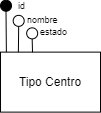
\includegraphics[scale=0.8]{img/diagramas/EER/E-TipoCentro.png}
        \caption{Entidad Tipo Centro}
        \label{fig:E-TipoCentro}
    \end{figure}

    \item Ejemplo de entidad (Tabla \ref{table:T-TipoCentro}):

    \begin{table}[H]
    \centering
        \begin{tabular}{ |p{6cm}||p{6cm}|  }
             \hline
                \multicolumn{2}{|c|}{\textbf{Tipo Centro}} \\
             \hline
                 \textbf{Atributo} & \textbf{Valor} \\
             \hline
                 id & 1 \\
             \hline
                 nombre & Facultad \\
             \hline
                 estado & 1 \\
        \end{tabular}
        \caption{Ejemplo de la entidad \textit{Tipo Centro}}
        \label{table:T-TipoCentro}
    \end{table}
\end{itemize}

\subsection{Entidad TipoRepresentaciónGobierno}
\begin{itemize}
    \item Descripción: este tipo de entidad representa a los tipos de miembros de gobierno registrados en el sistema que tienen vinculación con la Universidad de Córdoba. Los más destacados serían Director o Decano, Secretario, ViceDirectores o Vicedecanos, secretarios dirección...
    \item Restricciones: es una entidad fuerte por lo que no depende de otro tipo de entidad.
    \item Características:
    \begin{itemize}
        \item Nombre de la entidad: TipoRepresentaciónGobierno.
        \item Tipo: fuerte.
        \item Atributos heredados: ninguno.
        \item Atributo identificador primario: id.
        \item Atributo identificador alternativo: ninguno.
        \item Número de atributos: 3 (3 propios).
    \end{itemize}

    \item Atributos propios:
    \begin{itemize}
        \item id
        \begin{itemize}
            \item Definición: código numérico secuencial e incremental que identifica el tipo de centro.
            \item Dominio: números enteros mayores que 0.
            \item Tipo: clave primaria.
            \item Opcional: no
            \item Ejemplo: 5
        \end{itemize}

        \item nombre
        \begin{itemize}
            \item Definición: nombre que identifica al tipo de miembro de gobierno.
            \item Dominio: conjunto de 100 caracteres.
            \item Tipo: atributo simple.
            \item Opcional: no
            \item Ejemplo: Secretario
        \end{itemize}

        \item estado
        \begin{itemize}
            \item Definición: estado del tipo de representación del gobierno.
            \item Dominio: 1 (Habilitado), 0 (Deshabilitado).
            \item Tipo: atributo simple.
            \item Opcional: no
            \item Ejemplo: 1
        \end{itemize}
    \end{itemize}

    \item Diagrama (Figura \ref{fig:E-TipoRepresentaciónGobierno}):

    \begin{figure}[H]
        \centering
        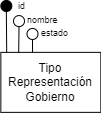
\includegraphics[scale=0.8]{img/diagramas/EER/E-TipoRepresentaciónGobierno.png}
        \caption{Entidad TipoRepresentaciónGobierno}
        \label{fig:E-TipoRepresentaciónGobierno}
    \end{figure}

    \item Ejemplo de entidad (Tabla \ref{table:T-TipoRepresentaciónGobierno}):

    \begin{table}[H]
    \centering
        \begin{tabular}{ |p{6cm}||p{6cm}|  }
             \hline
                \multicolumn{2}{|c|}{\textbf{TipoRepresentaciónGobierno}} \\
             \hline
                 \textbf{Atributo} & \textbf{Valor} \\
             \hline
                 id & 1 \\
             \hline
                 nombre & Secretario \\
             \hline
                 estado & 1 \\
        \end{tabular}
        \caption{Ejemplo de la entidad \textit{TipoRepresentaciónGobierno}}
        \label{table:T-TipoRepresentaciónGobierno}
    \end{table}
\end{itemize}

\subsection{Entidad TipoRepresentaciónGeneral}
\begin{itemize}
    \item Descripción: este tipo de entidad representa a los tipos de miembros de junta y comisión registrados en el sistema que tienen vinculación con la Universidad de Córdoba. Los más destacados serían Profesorado vinculación permanente, otro personal docente e investigador y  PAS, alumnado, personal libre designación...
    \item Restricciones: es una entidad fuerte por lo que no depende de otro tipo de entidad.
    \item Características:
    \begin{itemize}
        \item Nombre de la entidad: TipoRepresentaciónGeneral.
        \item Tipo: fuerte.
        \item Atributos heredados: ninguno.
        \item Atributo identificador primario: id.
        \item Atributo identificador alternativo: ninguno.
        \item Número de atributos: 3 (3 propios).
    \end{itemize}

    \item Atributos propios:
    \begin{itemize}
        \item id
        \begin{itemize}
            \item Definición: código numérico secuencial e incremental que identifica el tipo de centro.
            \item Dominio: números enteros mayores que 0.
            \item Tipo: clave primaria.
            \item Opcional: no
            \item Ejemplo: 5
        \end{itemize}

        \item nombre
        \begin{itemize}
            \item Definición: nombre que identifica al tipo de miembro de junta o comisión.
            \item Dominio: conjunto de 100 caracteres.
            \item Tipo: atributo simple.
            \item Opcional: no
            \item Ejemplo: PAS
        \end{itemize}

        \item estado
        \begin{itemize}
            \item Definición: estado del tipo de representación general.
            \item Dominio: 1 (Habilitado), 0 (Deshabilitado).
            \item Tipo: atributo simple.
            \item Opcional: no
            \item Ejemplo: 1
        \end{itemize}
    \end{itemize}

    \item Diagrama (Figura \ref{fig:E-TipoRepresentaciónGeneral}):

    \begin{figure}[H]
        \centering
        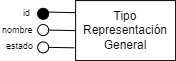
\includegraphics[scale=0.8]{img/diagramas/EER/E-TipoRepresentaciónGeneral.png}
        \caption{Entidad TipoRepresentaciónGeneral}
        \label{fig:E-TipoRepresentaciónGeneral}
    \end{figure}

    \item Ejemplo de entidad (Tabla \ref{table:T-TipoRepresentaciónGeneral}):

    \begin{table}[H]
    \centering
        \begin{tabular}{ |p{6cm}||p{6cm}|  }
             \hline
                \multicolumn{2}{|c|}{\textbf{TipoRepresentaciónGeneral}} \\
             \hline
                 \textbf{Atributo} & \textbf{Valor} \\
             \hline
                 id & 1 \\
             \hline
                 nombre & PAS \\
             \hline
                 estado & 1 \\
        \end{tabular}
        \caption{Ejemplo de la entidad \textit{TipoRepresentaciónGeneral}}
        \label{table:T-TipoRepresentaciónGeneral}
    \end{table}
\end{itemize}

\subsection{Entidad TipoConvocatoria}
\begin{itemize}
    \item Descripción: este tipo de entidad representa a los tipos de convocatorias de junta y comisión registrados en el sistema que tienen vinculación con la Universidad de Córdoba. Los más destacados serían oridnaria, extraordinaria y urgente.
    \item Restricciones: es una entidad fuerte por lo que no depende de otro tipo de entidad.
    \item Características:
    \begin{itemize}
        \item Nombre de la entidad: TipoConvocatoria.
        \item Tipo: fuerte.
        \item Atributos heredados: ninguno.
        \item Atributo identificador primario: id.
        \item Atributo identificador alternativo: ninguno.
        \item Número de atributos: 3 (3 propios).
    \end{itemize}

    \item Atributos propios:
    \begin{itemize}
        \item id
        \begin{itemize}
            \item Definición: código numérico secuencial e incremental que identifica el tipo de centro.
            \item Dominio: números enteros mayores que 0.
            \item Tipo: clave primaria.
            \item Opcional: no
            \item Ejemplo: 5
        \end{itemize}

        \item nombre
        \begin{itemize}
            \item Definición: nombre que identifica al tipo de convocatoria de junta o comisión.
            \item Dominio: conjunto de 100 caracteres.
            \item Tipo: atributo simple.
            \item Opcional: no
            \item Ejemplo: Ordinaria
        \end{itemize}

        \item estado
        \begin{itemize}
            \item Definición: estado del tipo de convocatoria.
            \item Dominio: 1 (Habilitado), 0 (Deshabilitado).
            \item Tipo: atributo simple.
            \item Opcional: no
            \item Ejemplo: 1
        \end{itemize}
    \end{itemize}

    \item Diagrama (Figura \ref{fig:E-TipoConvocatoria}):

    \begin{figure}[H]
        \centering
        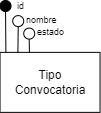
\includegraphics[scale=0.8]{img/diagramas/EER/E-TipoConvocatoria.png}
        \caption{Entidad TipoConvocatoria}
        \label{fig:E-TipoConvocatoria}
    \end{figure}

    \item Ejemplo de entidad (Tabla \ref{table:T-TipoConvocatoria}):

    \begin{table}[H]
    \centering
        \begin{tabular}{ |p{6cm}||p{6cm}|  }
             \hline
                \multicolumn{2}{|c|}{\textbf{TipoConvocatoria}} \\
             \hline
                 \textbf{Atributo} & \textbf{Valor} \\
             \hline
                 id & 1 \\
             \hline
                 nombre & Ordinaria \\
             \hline
                 estado & 1 \\
        \end{tabular}
        \caption{Ejemplo de la entidad \textit{TipoConvocatoria}}
        \label{table:T-TipoConvocatoria}
    \end{table}
\end{itemize}

\subsection{Entidad Usuario}
\begin{itemize}
    \item Descripción: este tipo de entidad representa a los usuarios registrados en el sistema que tienen vinculación con la Universidad de Córdoba.
    \item Restricciones: es una entidad fuerte por lo que no depende de otro tipo de entidad.
    \item Características:
    \begin{itemize}
        \item Nombre de la entidad: Usuario.
        \item Tipo: fuerte.
        \item Atributos heredados: ninguno.
        \item Atributo identificador primario: id.
        \item Atributo identificador alternativo: ninguno.
        \item Número de atributos: 5 propios.
    \end{itemize}

    \item Atributos propios:
    \begin{itemize}
        \item id
        \begin{itemize}
            \item Definición: código numérico secuencial e incremental que identifica el centro.
            \item Dominio: números enteros mayores que 0.
            \item Tipo: clave primaria.
            \item Opcional: no
            \item Ejemplo: 13
        \end{itemize}

        \item name
        \begin{itemize}
            \item Definición: nombre que identifica al usuario.
            \item Dominio: conjunto de 150 caracteres.
            \item Tipo: atributo simple.
            \item Opcional: no
            \item Ejemplo: Javier Ruiz
        \end{itemize}

        \item email
        \begin{itemize}
            \item Definición: dirección de correo del usuario.
            \item Dominio: conjunto de 250 caracteres.
            \item Tipo: atributo simple.
            \item Opcional: no
            \item Ejemplo: i03mosa@uco.es
        \end{itemize}

        \item password
        \begin{itemize}
            \item Definición: contraseña del usuario.
            \item Dominio: conjunto de 250 caracteres encriptados.
            \item Tipo: atributo simple.
            \item Opcional: no
            \item Ejemplo: 2y1092IXUNpkjO0rOQ5byMi
        \end{itemize}

        \item estado
        \begin{itemize}
            \item Definición: estado del usuario.
            \item Dominio: 1 (Habilitado), 0 (Deshabilitado).
            \item Tipo: atributo simple.
            \item Opcional: no
            \item Ejemplo: 1
        \end{itemize}
    \end{itemize}

    \item Diagrama (Figura \ref{fig:E-Usuario}):

    \begin{figure}[H]
        \centering
        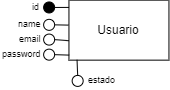
\includegraphics[scale=0.8]{img/diagramas/EER/E-Usuario.png}
        \caption{Entidad Usuario}
        \label{fig:E-Usuario}
    \end{figure}

    \item Ejemplo de entidad (Tabla \ref{table:T-Usuario}):

    \begin{table}[H]
    \centering
        \begin{tabular}{ |p{6cm}||p{6cm}|  }
             \hline
                \multicolumn{2}{|c|}{\textbf{Usuario}} \\
             \hline
                 \textbf{Atributo} & \textbf{Valor} \\
             \hline
                 id & 1 \\
             \hline
                 nombre & Ciencias \\
             \hline
                 email & i03mosa@uco.es \\
            \hline
                 password & 2y1092IXUNpkjO0rOQ5byMi \\
             \hline
                 estado & 1 \\
        \end{tabular}
        \caption{Ejemplo de la entidad \textit{Usuario}}
        \label{table:T-Usuario}
    \end{table}
\end{itemize}

\subsection{Entidad Centro}
\begin{itemize}
    \item Descripción: este tipo de entidad representa a los centros registrados en el sistema que tienen vinculación con la Universidad de Córdoba.
    \item Restricciones: es una entidad débil por identificación respecto de la entidad Tipo Centro.
    \item Características:
    \begin{itemize}
        \item Nombre de la entidad: Centro.
        \item Tipo: débil.
        \item Atributos heredados: idTipo, heredado de la entidad Tipo Centro.
        \item Atributo identificador primario: id.
        \item Atributo identificador alternativo: ninguno.
        \item Número de atributos: 5 (1 heredado y 4 propios).
    \end{itemize}

    \item Atributos propios:
    \begin{itemize}
        \item id
        \begin{itemize}
            \item Definición: código numérico secuencial e incremental que identifica el centro.
            \item Dominio: números enteros mayores que 0.
            \item Tipo: clave primaria.
            \item Opcional: no
            \item Ejemplo: 13
        \end{itemize}

        \item nombre
        \begin{itemize}
            \item Definición: nombre que identifica al centro.
            \item Dominio: conjunto de 150 caracteres.
            \item Tipo: atributo simple.
            \item Opcional: no
            \item Ejemplo: Javier Ruiz
        \end{itemize}

        \item dirección
        \begin{itemize}
            \item Definición: dirección donde se encuentra el centro.
            \item Dominio: conjunto de 250 caracteres.
            \item Tipo: atributo simple.
            \item Opcional: no
            \item Ejemplo: Campus de Rabanales
        \end{itemize}

        \item estado
        \begin{itemize}
            \item Definición: estado del centro.
            \item Dominio: 1 (Habilitado), 0 (Deshabilitado).
            \item Tipo: atributo simple.
            \item Opcional: no
            \item Ejemplo: 1
        \end{itemize}
    \end{itemize}

    \item Diagrama (Figura \ref{fig:E-Centro}):

    \begin{figure}[H]
        \centering
        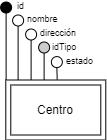
\includegraphics[scale=0.8]{img/diagramas/EER/E-Centro.png}
        \caption{Entidad Centro}
        \label{fig:E-Centro}
    \end{figure}

    \item Ejemplo de entidad (Tabla \ref{table:T-Centro}):

    \begin{table}[H]
    \centering
        \begin{tabular}{ |p{6cm}||p{6cm}|  }
             \hline
                \multicolumn{2}{|c|}{\textbf{Centro}} \\
             \hline
                 \textbf{Atributo} & \textbf{Valor} \\
             \hline
                 id & 1 \\
             \hline
                 nombre & Ciencias \\
             \hline
                 dirección & Campus Rabanales \\
             \hline
                 idTipo & 1 \\
             \hline
                 estado & 1 \\
        \end{tabular}
        \caption{Ejemplo de la entidad \textit{Centro}}
        \label{table:T-Centro}
    \end{table}
\end{itemize}

\subsection{Entidad Junta}
\begin{itemize}
    \item Descripción: este tipo de entidad representa a las juntas registradas en el sistema que tienen vinculación con la Universidad de Córdoba.
    \item Restricciones: es una entidad débil por identificación respecto de la entidad Centro.
    \item Características:
    \begin{itemize}
        \item Nombre de la entidad: Junta.
        \item Tipo: débil.
        \item Atributos heredados: idCentro, heredado de la entidad Centro.
        \item Atributo identificador primario: id.
        \item Atributo identificador alternativo: ninguno.
        \item Número de atributos: 5 (1 heredado y 4 propios).
    \end{itemize}

    \item Atributos propios:
    \begin{itemize}
        \item id
        \begin{itemize}
            \item Definición: código numérico secuencial e incremental que identifica la junta.
            \item Dominio: números enteros mayores que 0.
            \item Tipo: clave primaria.
            \item Opcional: no
            \item Ejemplo: 13
        \end{itemize}

        \item fechaConstitución
        \begin{itemize}
            \item Definición: fecha de creación de la junta.
            \item Dominio: 01/01/1970 hasta 31/12/9999.
            \item Tipo: atributo simple.
            \item Opcional: no
            \item Ejemplo: 10/09/2023
        \end{itemize}

        \item fechaDisolución
        \begin{itemize}
            \item Definición: fecha de disolución de la junta.
            \item Dominio: 01/01/1970 hasta 31/12/9999.
            \item Tipo: atributo simple.
            \item Opcional: sí
            \item Ejemplo: 10/09/2023
        \end{itemize}

        \item estado
        \begin{itemize}
            \item Definición: estado de la junta.
            \item Dominio: 1 (Habilitado), 0 (Deshabilitado).
            \item Tipo: atributo simple.
            \item Opcional: no
            \item Ejemplo: 1
        \end{itemize}
    \end{itemize}

    \item Diagrama (Figura \ref{fig:E-Junta}):

    \begin{figure}[H]
        \centering
        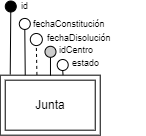
\includegraphics[scale=0.8]{img/diagramas/EER/E-Junta.png}
        \caption{Entidad Junta}
        \label{fig:E-Junta}
    \end{figure}

    \item Ejemplo de entidad (Tabla \ref{table:T-Junta}):

    \begin{table}[H]
    \centering
        \begin{tabular}{ |p{6cm}||p{6cm}|  }
             \hline
                \multicolumn{2}{|c|}{\textbf{Junta}} \\
             \hline
                 \textbf{Atributo} & \textbf{Valor} \\
             \hline
                 id & 1 \\
             \hline
                 fechaConstitución & 10/09/2023 \\
             \hline
                 fechaDisolución & 10/09/2027 \\
             \hline
                 idCentro & 1 \\
             \hline
                 estado & 1 \\
        \end{tabular}
        \caption{Ejemplo de la entidad \textit{Junta}}
        \label{table:T-Junta}
    \end{table}
\end{itemize}

\subsection{Entidad Comisión}
\begin{itemize}
    \item Descripción: este tipo de entidad representa a las comisiones registradas en el sistema que tienen vinculación con la Universidad de Córdoba.
    \item Restricciones: es una entidad débil por identificación respecto de la entidad Junta.
    \item Características:
    \begin{itemize}
        \item Nombre de la entidad: Comisión.
        \item Tipo: débil.
        \item Atributos heredados: idJunta, heredado de la entidad Junta.
        \item Atributo identificador primario: id.
        \item Atributo identificador alternativo: ninguno.
        \item Número de atributos: 7 (1 heredado y 6 propios).
    \end{itemize}

    \item Atributos propios:
    \begin{itemize}
        \item id
        \begin{itemize}
            \item Definición: código numérico secuencial e incremental que identifica la junta.
            \item Dominio: números enteros mayores que 0.
            \item Tipo: clave primaria.
            \item Opcional: no
            \item Ejemplo: 13
        \end{itemize}

         \item nombre
        \begin{itemize}
            \item Definición: nombre que identifica a la comisión.
            \item Dominio: conjunto de 100 caracteres.
            \item Tipo: atributo simple.
            \item Opcional: no
            \item Ejemplo: Asuntos económicos
        \end{itemize}

        \item descripción
        \begin{itemize}
            \item Definición: descripción de la comisión.
            \item Dominio: conjunto de 250 caracteres.
            \item Tipo: atributo simple.
            \item Opcional: no
            \item Ejemplo: Comisión dedicada a abordar todo lo referente a la economía de la comisión.
        \end{itemize}

        \item fechaConstitución
        \begin{itemize}
            \item Definición: fecha de creación de la junta.
            \item Dominio: 01/01/1970 hasta 31/12/9999.
            \item Tipo: atributo simple.
            \item Opcional: no
            \item Ejemplo: 10/09/2023
        \end{itemize}

        \item fechaDisolución
        \begin{itemize}
            \item Definición: fecha de disolución de la junta.
            \item Dominio: 01/01/1970 hasta 31/12/9999.
            \item Tipo: atributo simple.
            \item Opcional: sí
            \item Ejemplo: 10/09/2023
        \end{itemize}

        \item estado
        \begin{itemize}
            \item Definición: estado de la comisión.
            \item Dominio: 1 (Habilitado), 0 (Deshabilitado).
            \item Tipo: atributo simple.
            \item Opcional: no
            \item Ejemplo: 1
        \end{itemize}
    \end{itemize}

    \item Diagrama (Figura \ref{fig:E-Comisión}):

    \begin{figure}[H]
        \centering
        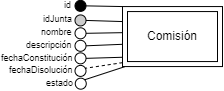
\includegraphics[scale=0.8]{img/diagramas/EER/E-Comisión.png}
        \caption{Entidad Comisión}
        \label{fig:E-Comisión}
    \end{figure}

    \item Ejemplo de entidad (Tabla \ref{table:T-Comisión}):

    \begin{table}[H]
    \centering
        \begin{tabular}{ |p{6cm}||p{6cm}|  }
             \hline
                \multicolumn{2}{|c|}{\textbf{Comisión}} \\
             \hline
                 \textbf{Atributo} & \textbf{Valor} \\
             \hline
                 id & 1 \\
             \hline
                 nombre & Asuntos económicos \\
            \hline
                 descripción & Comisión dedicada a abordar todo lo referente a la economía de la comisión \\
             \hline
                 fechaConstitución & 10/09/2023 \\
             \hline
                 fechaDisolución & 10/09/2027 \\
             \hline
                 idJunta & 1 \\
             \hline
                 estado & 1 \\
        \end{tabular}
        \caption{Ejemplo de la entidad \textit{Comisión}}
        \label{table:T-Comisión}
    \end{table}
\end{itemize}

\subsection{Entidad Convocatoria}
\begin{itemize}
    \item Descripción: este tipo de entidad representa a las convocatorias de comisión y junta registradas en el sistema.
    \item Restricciones: es una entidad débil por identificación respecto de la entidad TipoConvocatoria, la entidad Junta, la entidad Comisión.
    \item Características:
    \begin{itemize}
        \item Nombre de la entidad: Convocatoria.
        \item Tipo: débil.
        \item Atributos heredados: 
        \begin{itemize}
            \item idTipo, heredado de la entidad TipoConvocatoria. 
            \item idJun, heredado de la entidad Junta. 
            \item idCom, heredado de la entidad Comisión.
        \end{itemize}
        \item Atributo identificador primario: id.
        \item Atributo identificador alternativo: ninguno.
        \item Número de atributos: 9 (3 heredados y 6 propios).
    \end{itemize}

    \item Atributos propios:
    \begin{itemize}
        \item id
        \begin{itemize}
            \item Definición: código numérico secuencial e incremental que identifica la junta.
            \item Dominio: números enteros mayores que 0.
            \item Tipo: clave primaria.
            \item Opcional: no
            \item Ejemplo: 13
        \end{itemize}

         \item lugar
        \begin{itemize}
            \item Definición: lugar donde se celebrará la convocatoria.
            \item Dominio: conjunto de 100 caracteres.
            \item Tipo: atributo simple.
            \item Opcional: no
            \item Ejemplo: Rectorado UCO
        \end{itemize}

        \item fecha
        \begin{itemize}
            \item Definición: fecha en la que se celebrará la convocatoria.
            \item Dominio: 01/01/1970 hasta 31/12/9999.
            \item Tipo: atributo simple.
            \item Opcional: no
            \item Ejemplo: 10/09/2023
        \end{itemize}

         \item hora
        \begin{itemize}
            \item Definición: hora en la que se celebrará la convocatoria.
            \item Dominio: 00:00 hasta 23:59.
            \item Tipo: atributo simple.
            \item Opcional: no
            \item Ejemplo: 11:30
        \end{itemize}

        \item actaPDF
        \begin{itemize}
            \item Definición: ruta del documento PDF que contendrá información sobre la convocatoria celebrada.
            \item Dominio: conjunto de 200 caracteres.
            \item Tipo: atributo simple.
            \item Opcional: sí
            \item Ejemplo: /resources/convocatorias/1.pdf
        \end{itemize}

        \item estado
        \begin{itemize}
            \item Definición: estado de la convocatoria.
            \item Dominio: 1 (Habilitado), 0 (Deshabilitado).
            \item Tipo: atributo simple.
            \item Opcional: no
            \item Ejemplo: 1
        \end{itemize}
    \end{itemize}

    \item Diagrama (Figura \ref{fig:E-Convocatoria}):

    \begin{figure}[H]
        \centering
        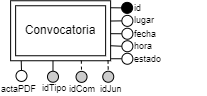
\includegraphics[scale=0.8]{img/diagramas/EER/E-Convocatoria.png}
        \caption{Entidad Convocatoria}
        \label{fig:E-Convocatoria}
    \end{figure}

    \item Ejemplo de entidad (Tabla \ref{table:T-Convocatoria}):

    \begin{table}[H]
    \centering
        \begin{tabular}{ |p{6cm}||p{6cm}|  }
             \hline
                \multicolumn{2}{|c|}{\textbf{Convocatoria}} \\
             \hline
                 \textbf{Atributo} & \textbf{Valor} \\
             \hline
                 id & 1 \\
             \hline
                 lugar & Rectorado UCO \\
            \hline
                 fecha & 10/09/2023 \\
             \hline
                 hora & 11:30 \\
             \hline
                 idTipo & 1 \\
             \hline
                 idJun & 1 \\
             \hline
                idCom &  \\
             \hline
                 estado & 1 \\
        \end{tabular}
        \caption{Ejemplo de la entidad \textit{Convocatoria}}
        \label{table:T-Convocatoria}
    \end{table}
\end{itemize}

\subsection{Entidad MiembroGobierno}
\begin{itemize}
    \item Descripción: este tipo de entidad representa a los miembros del equipo de gobierno de cada centro registrados en el sistema que tienen vinculación con la Universidad de Córdoba.
    \item Restricciones: es una entidad débil por identificación respecto de la entidad Usuario, la entidad Centro y la entidad TipoRepresentaciónGobierno.
    \item Características:
    \begin{itemize}
        \item Nombre de la entidad: MiembroGobierno.
        \item Tipo: débil.
        \item Atributos heredados: 
        \begin{itemize}
            \item idUsuario, heredado de la entidad Usuario.
            \item idCentro, heredado de la entidad Centro.
            \item idRepresentacion, heredado de la entidad TipoRepresentaciónGobierno.
        \end{itemize} 
        \item Atributo identificador primario: id.
        \item Atributo identificador alternativo: ninguno.
        \item Número de atributos: 6 (3 heredados y 3 propios).
    \end{itemize}

    \item Atributos propios:
    \begin{itemize}
        \item id
        \begin{itemize}
            \item Definición: código numérico secuencial e incremental que identifica la junta.
            \item Dominio: números enteros mayores que 0.
            \item Tipo: clave primaria.
            \item Opcional: no
            \item Ejemplo: 13
        \end{itemize}

        \item fechaTomaPosesión
        \begin{itemize}
            \item Definición: fecha de toma de posesión del miembro de gobierno.
            \item Dominio: 01/01/1970 hasta 31/12/9999.
            \item Tipo: atributo simple.
            \item Opcional: no
            \item Ejemplo: 10/09/2023
        \end{itemize}

        \item fechaCese
        \begin{itemize}
            \item Definición: fecha de cese del miembro de gobierno.
            \item Dominio: 01/01/1970 hasta 31/12/9999.
            \item Tipo: atributo simple.
            \item Opcional: sí
            \item Ejemplo: 10/09/2023
        \end{itemize}

        \item estado
        \begin{itemize}
            \item Definición: estado del miembro del gobierno.
            \item Dominio: 1 (Habilitado), 0 (Deshabilitado).
            \item Tipo: atributo simple.
            \item Opcional: no
            \item Ejemplo: 1
        \end{itemize}
    \end{itemize}

    \item Diagrama (Figura \ref{fig:E-MiembroGobierno}):

    \begin{figure}[H]
        \centering
        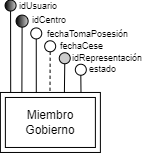
\includegraphics[scale=0.8]{img/diagramas/EER/E-MiembroGobierno.png}
        \caption{Entidad MiembroGobierno}
        \label{fig:E-MiembroGobierno}
    \end{figure}

    \item Ejemplo de entidad (Tabla \ref{table:T-MiembroGobierno}):

    \begin{table}[H]
    \centering
        \begin{tabular}{ |p{6cm}||p{6cm}|  }
             \hline
                \multicolumn{2}{|c|}{\textbf{MiembroGobierno}} \\
             \hline
                 \textbf{Atributo} & \textbf{Valor} \\
             \hline
                 id & 1 \\
             \hline
                 fechaTomaPosesión & 10/09/2023 \\
             \hline
                 fechaCese & 10/09/2027 \\
             \hline
                 idUsuario & 1 \\
             \hline
                 idCentro & 1 \\
            \hline
                 idRepresentación & 1 \\
             \hline
                 estado & 1 \\
        \end{tabular}
        \caption{Ejemplo de la entidad \textit{MiembroGobierno}}
        \label{table:T-MiembroGobierno}
    \end{table}
\end{itemize}

\subsection{Entidad MiembroJunta}
\begin{itemize}
    \item Descripción: este tipo de entidad representa a los miembros de la junta de cada centro registrados en el sistema que tienen vinculación con la Universidad de Córdoba.
    \item Restricciones: es una entidad débil por identificación respecto de la entidad Usuario, la entidad Junta y la entidad TipoRepresentaciónGeneral.
    \item Características:
    \begin{itemize}
        \item Nombre de la entidad: MiembroJunta.
        \item Tipo: débil.
        \item Atributos heredados: 
        \begin{itemize}
            \item idUsuario, heredado de la entidad Usuario.
            \item idJunta, heredado de la entidad Junta.
            \item idRepresentacion, heredado de la entidad TipoRepresentaciónGeneral.
        \end{itemize} 
        \item Atributo identificador primario: id.
        \item Atributo identificador alternativo: ninguno.
        \item Número de atributos: 6 (3 heredados y 3 propios).
    \end{itemize}

    \item Atributos propios:
    \begin{itemize}
        \item id
        \begin{itemize}
            \item Definición: código numérico secuencial e incremental que identifica la junta.
            \item Dominio: números enteros mayores que 0.
            \item Tipo: clave primaria.
            \item Opcional: no
            \item Ejemplo: 13
        \end{itemize}

        \item fechaTomaPosesión
        \begin{itemize}
            \item Definición: fecha de toma de posesión del miembro de gobierno.
            \item Dominio: 01/01/1970 hasta 31/12/9999.
            \item Tipo: atributo simple.
            \item Opcional: no
            \item Ejemplo: 10/09/2023
        \end{itemize}

        \item fechaCese
        \begin{itemize}
            \item Definición: fecha de cese del miembro de gobierno.
            \item Dominio: 01/01/1970 hasta 31/12/9999.
            \item Tipo: atributo simple.
            \item Opcional: sí
            \item Ejemplo: 10/09/2023
        \end{itemize}

        \item estado
        \begin{itemize}
            \item Definición: estado del miembro de la junta.
            \item Dominio: 1 (Habilitado), 0 (Deshabilitado).
            \item Tipo: atributo simple.
            \item Opcional: no
            \item Ejemplo: 1
        \end{itemize}
    \end{itemize}

    \item Diagrama (Figura \ref{fig:E-MiembroJunta}):

    \begin{figure}[H]
        \centering
        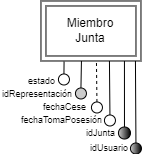
\includegraphics[scale=0.8]{img/diagramas/EER/E-MiembroJunta.png}
        \caption{Entidad MiembroJunta}
        \label{fig:E-MiembroJunta}
    \end{figure}

    \item Ejemplo de entidad (Tabla \ref{table:T-MiembroJunta}):

    \begin{table}[H]
    \centering
        \begin{tabular}{ |p{6cm}||p{6cm}|  }
             \hline
                \multicolumn{2}{|c|}{\textbf{MiembroJunta}} \\
             \hline
                 \textbf{Atributo} & \textbf{Valor} \\
             \hline
                 id & 1 \\
             \hline
                 fechaTomaPosesión & 10/09/2023 \\
             \hline
                 fechaCese & 10/09/2027 \\
             \hline
                 idUsuario & 1 \\
             \hline
                 idJunta & 1 \\
            \hline
                 idRepresentación & 1 \\
             \hline
                 estado & 1 \\
        \end{tabular}
        \caption{Ejemplo de la entidad \textit{MiembroJunta}}
        \label{table:T-MiembroJunta}
    \end{table}
\end{itemize}

\subsection{Entidad MiembroComisión}
\begin{itemize}
    \item Descripción: este tipo de entidad representa a los miembros de la comisión de cada junta de cada centro registrados en el sistema que tienen vinculación con la Universidad de Córdoba.
    \item Restricciones: es una entidad débil por identificación respecto de la entidad Usuario, la entidad Comsii¡sión y la entidad TipoRepresentaciónGeneral.
    \item Características:
    \begin{itemize}
        \item Nombre de la entidad: MiembroComisión.
        \item Tipo: débil.
        \item Atributos heredados: 
        \begin{itemize}
            \item idUsuario, heredado de la entidad Usuario.
            \item idComisión, heredado de la entidad Comisión.
            \item idRepresentacion, heredado de la entidad TipoRepresentaciónGeneral.
        \end{itemize} 
        \item Atributo identificador primario: id.
        \item Atributo identificador alternativo: ninguno.
        \item Número de atributos: 6 (3 heredados y 3 propios).
    \end{itemize}

    \item Atributos propios:
    \begin{itemize}
        \item id
        \begin{itemize}
            \item Definición: código numérico secuencial e incremental que identifica la junta.
            \item Dominio: números enteros mayores que 0.
            \item Tipo: clave primaria.
            \item Opcional: no
            \item Ejemplo: 13
        \end{itemize}

        \item fechaTomaPosesión
        \begin{itemize}
            \item Definición: fecha de toma de posesión del miembro de gobierno.
            \item Dominio: 01/01/1970 hasta 31/12/9999.
            \item Tipo: atributo simple.
            \item Opcional: no
            \item Ejemplo: 10/09/2023
        \end{itemize}

        \item fechaCese
        \begin{itemize}
            \item Definición: fecha de cese del miembro de gobierno.
            \item Dominio: 01/01/1970 hasta 31/12/9999.
            \item Tipo: atributo simple.
            \item Opcional: sí
            \item Ejemplo: 10/09/2023
        \end{itemize}

        \item estado
        \begin{itemize}
            \item Definición: estado del miembro de la comisión.
            \item Dominio: 1 (Habilitado), 0 (Deshabilitado).
            \item Tipo: atributo simple.
            \item Opcional: no
            \item Ejemplo: 1
        \end{itemize}
    \end{itemize}

    \item Diagrama (Figura \ref{fig:E-MiembroComisión}):

    \begin{figure}[H]
        \centering
        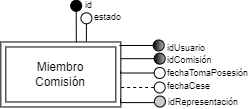
\includegraphics[scale=0.8]{img/diagramas/EER/E-MiembroComisión.png}
        \caption{Entidad MiembroComisión}
        \label{fig:E-MiembroComisión}
    \end{figure}

    \item Ejemplo de entidad (Tabla \ref{table:T-MiembroComisión}):

    \begin{table}[H]
    \centering
        \begin{tabular}{ |p{6cm}||p{6cm}|  }
             \hline
                \multicolumn{2}{|c|}{\textbf{MiembroComisión}} \\
             \hline
                 \textbf{Atributo} & \textbf{Valor} \\
             \hline
                 id & 1 \\
             \hline
                 fechaTomaPosesión & 10/09/2023 \\
             \hline
                 fechaCese & 10/09/2027 \\
             \hline
                 idUsuario & 1 \\
             \hline
                 idComisión & 1 \\
            \hline
                 idRepresentación & 1 \\
             \hline
                 estado & 1 \\
        \end{tabular}
        \caption{Ejemplo de la entidad \textit{MiembroComisión}}
        \label{table:T-MiembroComisión}
    \end{table}
\end{itemize}


\section{Tipos de interrelación} \label{sec:relaciones}
En esta sección se identificarán y describirán las interrelaciones entre los tipos de entidad descritos en la sección 7.2.

Las interrelaciones pueden ser de tipo débil o fuerte.

\begin{itemize}
    \item Un tipo de Interrelación Fuerte es aquella que representa la relación existente entre dos tipos de entidad fuertes.

    \item Un tipo de Interrelación Débil es aquella que representa la relación entre un tipo de entidad débil y otro fuerte o entre dos tipos de entidad débiles.
\end{itemize}

De acuerdo con la notación del modelo E-R, una interrelación se representa mediante un rombo del que parten flechas hacia los tipos de entidad que forman parte de la relación. Cada tipo de entidad interviene en la interrelación con una determinada cardinalidad, que indica el número mínimo y máximo de instancias de cada tipo de entidad que pueden participar en la interrelación. Se representa por dos valores entre paréntesis (mínimo y máximo). Las posibles cardinalidades son: (0,1), (1,1),(0,n),(1,n),(m,n). Estas cardinalidades determinan el tipo de interrelación que se está definiendo, que puede ser:

\begin{itemize}
    \item \textbf{1:1} Uno a uno. Cuando los dos tipos de entidad participan con una cardinalidad máxima de 1.
    \item \textbf{1:N o N:1} Uno a muchos, o muchos a uno. Cuando uno de los tipos de entidad participa con una cardinalidad máxima de 1 y el otro con una cardinalidad máxima de n.
    \item \textbf{N:N} Muchos a muchos. Cuando ambos tipos de entidad participan una cardinalidad máxima de n.
\end{itemize}

Para cada una de las interrelaciones que se han identificado en la definición del problema, se indicará la siguiente información:

\begin{itemize}
    \item \textbf{Nombre}. Nombre del tipo de interrelación.
    \item \textbf{Descripción}. Definición del tipo de interrelación y de los tipos de entidad que participan en ella.
    \item \textbf{Tipo}. Indicación de si se trata de un tipo de interrelación débil o fuerte identificando los tipos de debilidad en su caso.
    \item \textbf{Cardinalidad}. Indicación de la cardinalidad del tipo de interrelación y cardinalidades mínima y máxima de los tipos de entidad intervinientes.
    \item \textbf{Atributos}. Indicación del número y descripción de los atributos del tipo de interrelación, en su caso.
    \item \textbf{Diagrama}. Representación gráfica del tipo de interrelación, de acuerdo con la notación E-R.
    \item \textbf{Ejemplo}. Valores de muestra.
\end{itemize}

Se han identificado las interrelaciones que se indican a continuación y que se describirán en las siguientes subsecciones:

\begin{itemize}
    \item Tipo de Interrelación: TipoCentro - Centro.
    \item Tipo de Interrelación: TipoRepresentaciónGobierno - MiembroGobierno.
    \item Tipo de Interrelación: TipoRepresentaciónGeneral - MiembroJunta.
    \item Tipo de Interrelación: TipoRepresentaciónGeneral - MiembroComisión.
    \item Tipo de Interrelación: TipoConvocatoria - Convocatoria.
    \item Tipo de Interrelación: Centro - MiembroGobierno.
    \item Tipo de Interrelación: Centro - Junta.
    \item Tipo de Interrelación: Junta - MiembroJunta.
    \item Tipo de Interrelación: Junta - Comisión.
    \item Tipo de Interrelación: Junta - Convocatoria.
    \item Tipo de Interrelación: Comisión - MiembroComisión.
    \item Tipo de Interrelación: Comisión - Convocatoria.
    \item Tipo de Interrelación: Usuario - MiembroGobierno.
    \item Tipo de Interrelación: Usuario - MiembroJunta.
    \item Tipo de Interrelación: Usuario - MiembroComisión.
\end{itemize}

\subsection{Interrelación: TipoCentro - Centro}
\begin{itemize}
    \item \textbf{Nombre}: TipCt-Ct.
    \item \textbf{Descripción}: esta interrelación muestra que un tipo de centro puede corresponder a cero, uno o más centros, pero un centro solamente tiene un tipo de centro.
    \item \textbf{Tipo}: la entidad Centro presenta una debilidad por identificación respecto de la entidad Tipo Centro.
    \item \textbf{Cardinalidad}. 1:N
    \begin{itemize}
        \item Cardinalidad de TipoCentro (0,n): un tipo de centro puede tener asociadas 0, 1 o varios centros.
        \item Cardinalidad de Centro (1,1): un centro solamente está asociado a un tipo de centro.
    \end{itemize}
    \item \textbf{Atributos}: ninguno
    \item \textbf{Diagrama} (Figura \ref{fig:I-TipCt-Ct}) 
    \begin{figure}[H]
        \centering
        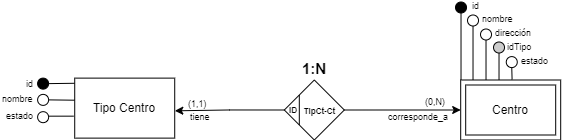
\includegraphics[scale=0.7]{img/diagramas/EER/I-TipCt-Ct.png}
        \caption{Interrelación: TipoCentro - Centro}
        \label{fig:I-TipCt-Ct}
    \end{figure}
    
    \item \textbf{Ejemplo} (Tabla \ref{table:I-TipCt-Ct}).

    \begin{table}[H]
    \centering
        \begin{tabular}{ | c | c | c |  }
             \hline
                 \textbf{Entidad} & \textbf{Atributo} & \textbf{Ejemplo}\\       
             \hline
                 \textbf{Tipo Centro}  & \underline{id} & 1\\
                  & nombre & Facultad\\
                  & estado & 1\\
             \hline
                 \textbf{Centro}  & \underline{id} & 1\\
                  & nombre & Ciencias\\
                  & dirección & Campus de Rabanales\\
                  & idTipo & 1\\
                  & estado & 1\\
        \end{tabular}
        \caption{Ejemplo de la interrelación \textit{TipoCentro - Centro}}
        \label{table:I-TipCt-Ct}
    \end{table}

\end{itemize}

\subsection{Interrelación: TipoRepresentaciónGobierno - MiembroGobierno }
\begin{itemize}
    \item \textbf{Nombre}: TipGob-MiGob.
    \item \textbf{Descripción}: esta interrelación muestra que un tipo de representación de gobierno puede corresponder a cero, uno o más miembros de gobierno, pero un miembro de gobierno solamente tiene un tipo de representación de gobierno.
    \item \textbf{Tipo}: la entidad Miembro Gobierno presenta una debilidad por identificación respecto de la entidad Tipo Representación Gobierno.
    \item \textbf{Cardinalidad}. 1:N
    \begin{itemize}
        \item Cardinalidad de TipoRepresentaciónGobierno (0,n): un tipo de representación gobierno puede tener asociadas 0, 1 o varios miembros de gobierno.
        \item Cardinalidad de MiembroGobierno (1,1): un miembro de gobierno solamente está asociado a un tipo de representación de gobierno.
    \end{itemize}
    \item \textbf{Atributos}: ninguno
    \item \textbf{Diagrama} (Figura \ref{fig:I-TipGob-MiGob}) 
    \begin{figure}[H]
        \centering
        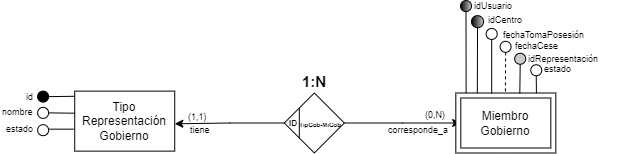
\includegraphics[scale=0.7]{img/diagramas/EER/I-TipGob-MiGob.png}
        \caption{Interrelación: TipoRepresentaciónGobierno - MiembroGobierno}
        \label{fig:I-TipGob-MiGob}
    \end{figure}
    
    \item \textbf{Ejemplo} (Tabla \ref{table:I-TipGob-MiGob}).

    \begin{table}[H]
    \centering
        \begin{tabular}{ | c | c | c |  }
             \hline
                 \textbf{Entidad} & \textbf{Atributo} & \textbf{Ejemplo}\\       
             \hline
                 \textbf{Tipo Representación Gobierno}  & \underline{id} & 1\\
                  & nombre & Director\\
                  & estado & 1\\
             \hline
                 \textbf{Miembro Gobierno}  & \underline{id} & 1\\
                  & idUsuario & 1\\
                  & idCentro & 1\\
                  & idRepresentación & 1\\
                  & fechaTomaPosesión & 10/09/2023\\
                  & fechaCese & null\\
                  & estado & 1\\
        \end{tabular}
        \caption{Ejemplo de la interrelación \textit{TipoRepresentaciónGobierno - MiembroGobierno}}
        \label{table:I-TipGob-MiGob}
    \end{table}
\end{itemize}

\subsection{Interrelación: TipoRepresentaciónGeneral - MiembroJunta}
\begin{itemize}
    \item \textbf{Nombre}: TipRG-MiJu.
    \item \textbf{Descripción}: esta interrelación muestra que un tipo de representación general puede corresponder a cero, uno o más miembros de junta, pero un miembro de junta solamente tiene un tipo de representación general.
    \item \textbf{Tipo}: la entidad Miembro Junta presenta una debilidad por identificación respecto de la entidad Tipo Representación General.
    \item \textbf{Cardinalidad}. 1:N
    \begin{itemize}
        \item Cardinalidad de TipoRepresentaciónGeneral (0,n): un tipo de representación general puede tener asociadas 0, 1 o varios miembros de junta.
        \item Cardinalidad de MiembroJunta (1,1): un miembro de junta solamente está asociado a un tipo de representación general.
    \end{itemize}
    \item \textbf{Atributos}: ninguno
    \item \textbf{Diagrama} (Figura \ref{fig:I-TipRG-MiJu}) 
    \begin{figure}[H]
        \centering
        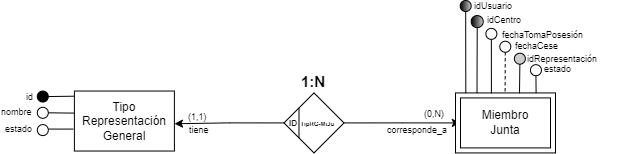
\includegraphics[scale=0.7]{img/diagramas/EER/I-TipRG-MiJu.png}
        \caption{Interrelación: TipoRepresentaciónGeneral - MiembroJunta}
        \label{fig:I-TipRG-MiJu}
    \end{figure}
    
    \item \textbf{Ejemplo} (Tabla \ref{table:I-TipRG-MiJu}).

    \begin{table}[H]
    \centering
        \begin{tabular}{ | c | c | c |  }
             \hline
                 \textbf{Entidad} & \textbf{Atributo} & \textbf{Ejemplo}\\       
             \hline
                 \textbf{Tipo Representación General}  & \underline{id} & 1\\
                  & nombre & Profesorado vinculación permanente\\
                  & estado & 1\\
             \hline
                 \textbf{Miembro Junta}  & \underline{id} & 1\\
                  & idUsuario & 1\\
                  & idJunta & 1\\
                  & idRepresentación & 1\\
                  & fechaTomaPosesión & 10/09/2023\\
                  & fechaCese & null\\
                  & estado & 1\\
        \end{tabular}
        \caption{Ejemplo de la interrelación \textit{TipoRepresentaciónGeneral - MiembroJunta}}
        \label{table:I-TipRG-MiJu}
    \end{table}
\end{itemize}

\subsection{Interrelación: TipoRepresentaciónGeneral - MiembroComisión}
\begin{itemize}
    \item \textbf{Nombre}: TipRG-MiCom.
    \item \textbf{Descripción}: esta interrelación muestra que un tipo de representación general puede corresponder a cero, uno o más miembros de comisión, pero un miembro de comisión solamente tiene un tipo de representación general.
    \item \textbf{Tipo}: la entidad Miembro Comisión presenta una debilidad por identificación respecto de la entidad Tipo Representación General.
    \item \textbf{Cardinalidad}. 1:N
    \begin{itemize}
        \item Cardinalidad de TipoRepresentaciónGeneral (0,n): un tipo de representación general puede tener asociadas 0, 1 o varios miembros de comisión.
        \item Cardinalidad de MiembroComisión (1,1): un miembro de comisión solamente está asociado a un tipo de representación general.
    \end{itemize}
    \item \textbf{Atributos}: ninguno
    \item \textbf{Diagrama} (Figura \ref{fig:I-TipRG-MiCom}) 
    \begin{figure}[H]
        \centering
        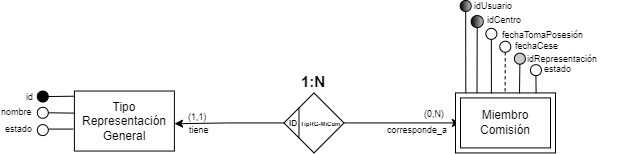
\includegraphics[scale=0.7]{img/diagramas/EER/I-TipRG-MiCom.png}
        \caption{Interrelación: TipoRepresentaciónGeneral - MiembroComisión}
        \label{fig:I-TipRG-MiCom}
    \end{figure}
    
    \item \textbf{Ejemplo} (Tabla \ref{table:I-TipRG-MiCom}).

    \begin{table}[H]
    \centering
        \begin{tabular}{ | c | c | c |  }
             \hline
                 \textbf{Entidad} & \textbf{Atributo} & \textbf{Ejemplo}\\       
             \hline
                 \textbf{Tipo Representación General}  & \underline{id} & 2\\
                  & nombre & PAS\\
                  & estado & 1\\
             \hline
                 \textbf{Miembro Comisión}  & \underline{id} & 1\\
                  & idUsuario & 1\\
                  & idComisión & 1\\
                  & idRepresentación & 2\\
                  & fechaTomaPosesión & 10/09/2023\\
                  & fechaCese & null\\
                  & estado & 1\\
        \end{tabular}
        \caption{Ejemplo de la interrelación \textit{TipoRepresentaciónGeneral - MiembroComisión}}
        \label{table:I-TipRG-MiCom}
    \end{table}
\end{itemize}

\subsection{Interrelación: TipoConvocatoria - Convocatoria}
\begin{itemize}
    \item \textbf{Nombre}: TipConv-Conv.
    \item \textbf{Descripción}: esta interrelación muestra que un tipo de convocatoria puede corresponder a cero, uno o más convocatorias, pero una convocatoria solamente tiene un tipo de convocatoria.
    \item \textbf{Tipo}: la entidad Convocatoria presenta una debilidad por identificación respecto de la entidad Tipo Convocatoria.
    \item \textbf{Cardinalidad}. 1:N
    \begin{itemize}
        \item Cardinalidad de Tipo Convocatoria (0,n): un tipo de convocatoria puede tener asociadas 0, 1 o varias convocatorias.
        \item Cardinalidad de Convocatoria (1,1): una convocatoria solamente está asociada a un tipo de convocatoria.
    \end{itemize}
    \item \textbf{Atributos}: ninguno
    \item \textbf{Diagrama} (Figura \ref{fig:I-TipConv-Conv}) 
    \begin{figure}[H]
        \centering
        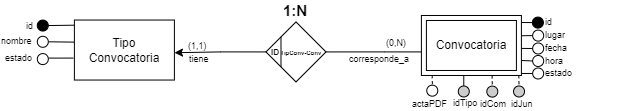
\includegraphics[scale=0.7]{img/diagramas/EER/I-TipConv-Conv.png}
        \caption{Interrelación: TipoConvocatoria - Convocatoria}
        \label{fig:I-TipConv-Conv}
    \end{figure}
    
    \item \textbf{Ejemplo} (Tabla \ref{table:I-TipConv-Conv}).

    \begin{table}[H]
    \centering
        \begin{tabular}{ | c | c | c |  }
             \hline
                 \textbf{Entidad} & \textbf{Atributo} & \textbf{Ejemplo}\\       
             \hline
                 \textbf{Tipo Convocvatoria}  & \underline{id} & 1\\
                  & nombre & Ordinaria\\
                  & estado & 1\\
             \hline
                 \textbf{Convocatoria}  & \underline{id} & 1\\
                  & lugar & Rectorado\\
                  & fecha & 23/09/2023\\
                  & hora & 11:30\\
                  & idTipo & 1\\
                  & idComision & null\\
                  & idJunta & 1\\
                  & acta & /resources/actas/1.pdf \\
                  & estado & 1\\
        \end{tabular}
        \caption{Ejemplo de la interrelación \textit{TipoConvocatoria - Convocatoria}}
        \label{table:I-TipConv-Conv}
    \end{table}
\end{itemize}

\subsection{Interrelación: Centro - MiembroGobierno}
\begin{itemize}
    \item \textbf{Nombre}: Ct-MiGob.
    \item \textbf{Descripción}: esta interrelación muestra que un centro puede ser representado por uno o más miembros de gobierno, pero un miembro de gobierno solamente representa un centro.
    \item \textbf{Tipo}: la entidad MiembroGobierno presenta una debilidad por identificación respecto de la entidad Centro.
    \item \textbf{Cardinalidad}. 1:N
    \begin{itemize}
        \item Cardinalidad de Centro (1,n): un centro puede tener asociados 1 o varias miembros de gobierno.
        \item Cardinalidad de MiembroGobierno (1,1): un miembro de gobierno solamente está asociado a un centro.
    \end{itemize}
    \item \textbf{Atributos}: ninguno
    \item \textbf{Diagrama} (Figura \ref{fig:I-Ct-MiGob}) 
    \begin{figure}[H]
        \centering
        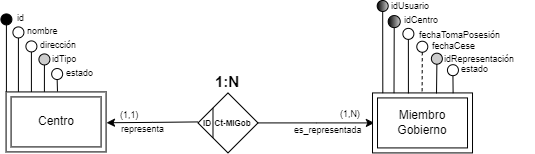
\includegraphics[scale=0.7]{img/diagramas/EER/I-Ct-MiGob.png}
        \caption{Interrelación: Centro - MiembroGobierno}
        \label{fig:I-Ct-MiGob}
    \end{figure}
    
    \item \textbf{Ejemplo} (Tabla \ref{table:I-Ct-MiGob}).

    \begin{table}[H]
    \centering
        \begin{tabular}{ | c | c | c |  }
             \hline
                 \textbf{Entidad} & \textbf{Atributo} & \textbf{Ejemplo}\\       
             \hline
                 \textbf{Centro}  & \underline{id} & 1\\
                  & nombre & Ciencias\\
                  & dirección & Campus de Rabanales\\
                  & idTipo & 1\\
                  & estado & 1\\
             \hline
                 \textbf{Miembro Gobierno}  & \underline{id} & 1\\
                  & idUsuario & 1\\
                  & idCentro & 1\\
                  & idRepresentación & 1\\
                  & fechaTomaPosesión & 10/09/2023\\
                  & fechaCese & null\\
                  & estado & 1\\
        \end{tabular}
        \caption{Ejemplo de la interrelación \textit{Centro - MiembroGobierno}}
        \label{table:I-Ct-MiGob}
    \end{table}
\end{itemize}

\subsection{Interrelación: Centro - Junta}
\begin{itemize}
    \item \textbf{Nombre}: Ct-Ju.
    \item \textbf{Descripción}: esta interrelación muestra que un centro puede ser coordinado por cero, uno o más juntas, pero una junta solamente coordina un centro.
    \item \textbf{Tipo}: la entidad Junta presenta una debilidad por identificación respecto de la entidad Centro.
    \item \textbf{Cardinalidad}. 1:N
    \begin{itemize}
        \item Cardinalidad de Centro (0,n): un centro puede tener asociados 0, 1 o varias juntas.
        \item Cardinalidad de Junta (1,1): una junta solamente está asociada a un centro.
    \end{itemize}
    \item \textbf{Atributos}: ninguno
    \item \textbf{Diagrama} (Figura \ref{fig:I-Ct-Ju}) 
    \begin{figure}[H]
        \centering
        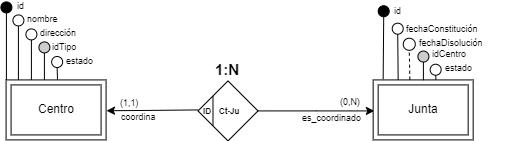
\includegraphics[scale=0.7]{img/diagramas/EER/I-Ct-Ju}
        \caption{Interrelación: Centro - Junta}
        \label{fig:I-Ct-Ju}
    \end{figure}
    
    \item \textbf{Ejemplo} (Tabla \ref{table:I-Ct-Ju}).

    \begin{table}[H]
    \centering
        \begin{tabular}{ | c | c | c |  }
             \hline
                 \textbf{Entidad} & \textbf{Atributo} & \textbf{Ejemplo}\\       
             \hline
                 \textbf{Centro}  & \underline{id} & 1\\
                  & nombre & Ciencias\\
                  & dirección & Campus de Rabanales\\
                  & idTipo & 1\\
                  & estado & 1\\
             \hline
                 \textbf{Junta}  & \underline{id} & 1\\
                  & idCentro & 1\\
                  & fechaConstitución & 10/09/2023\\
                  & fechaDisolución & null\\
                  & estado & 1\\
        \end{tabular}
        \caption{Ejemplo de la interrelación \textit{Centro - Junta}}
        \label{table:I-Ct-Ju}
    \end{table}
\end{itemize}

\subsection{Interrelación: Junta - MiembroJunta}
\begin{itemize}
    \item \textbf{Nombre}: Ju-MiJu.
    \item \textbf{Descripción}: esta interrelación muestra que una junta puede ser representada por cero, uno o más miembros de junta, pero un miembro de junta solamente representa una junta.
    \item \textbf{Tipo}: la entidad MiembroJunta presenta una debilidad por identificación respecto de la entidad Junta.
    \item \textbf{Cardinalidad}. 1:N
    \begin{itemize}
        \item Cardinalidad de Junta (0,n): una junta puede tener asociados 0, 1 o varios miembros de junta.
        \item Cardinalidad de MiembroJunta (1,1): un miembro de junta solamente está asociado a una junta.
    \end{itemize}
    \item \textbf{Atributos}: ninguno
    \item \textbf{Diagrama} (Figura \ref{fig:I-Ju-MiJu}) 
    \begin{figure}[H]
        \centering
        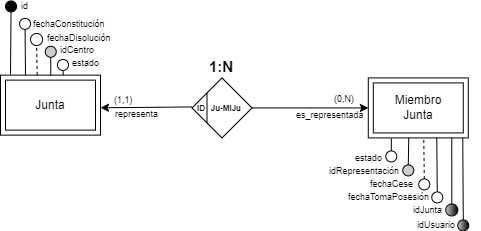
\includegraphics[scale=0.7]{img/diagramas/EER/I-Ju-MiJu}
        \caption{Interrelación: Junta - MiembroJunta}
        \label{fig:I-Ju-MiJu}
    \end{figure}
    
    \item \textbf{Ejemplo} (Tabla \ref{table:I-Ju-MiJu}).

    \begin{table}[H]
    \centering
        \begin{tabular}{ | c | c | c |  }
             \hline
                 \textbf{Entidad} & \textbf{Atributo} & \textbf{Ejemplo}\\       
             \hline
                 \textbf{Junta}  & \underline{id} & 1\\
                  & idCentro & 1\\
                  & fechaConstitución & 10/09/2023\\
                  & fechaDisolución & null\\
                  & estado & 1\\
              \hline
                 \textbf{Miembro Junta}  & \underline{id} & 1\\
                  & idUsuario & 1\\
                  & idJunta & 1\\
                  & idRepresentación & 1\\
                  & fechaTomaPosesión & 10/09/2023\\
                  & fechaCese & null\\
                  & estado & 1\\
        \end{tabular}
        \caption{Ejemplo de la interrelación \textit{Junta - MiembroJunta}}
        \label{table:I-Ju-MiJu}
    \end{table}
\end{itemize}

\subsection{Interrelación: Junta - Comisión}
\begin{itemize}
    \item \textbf{Nombre}: Ju-Com.
    \item \textbf{Descripción}: esta interrelación muestra que una junta puede gestionar cero, uno o más comisiones, pero una comisión solamente puede ser gestionada por una junta.
    \item \textbf{Tipo}: la entidad Comisión presenta una debilidad por identificación respecto de la entidad Junta.
    \item \textbf{Cardinalidad}. 1:N
    \begin{itemize}
        \item Cardinalidad de Junta (0,n): una junta puede tener asociados 0, 1 o varias comisiones.
        \item Cardinalidad de Comisión (1,1): una comisión solamente está asociado a una junta.
    \end{itemize}
    \item \textbf{Atributos}: ninguno
    \item \textbf{Diagrama} (Figura \ref{fig:I-Ju-Com}) 
    \begin{figure}[H]
        \centering
        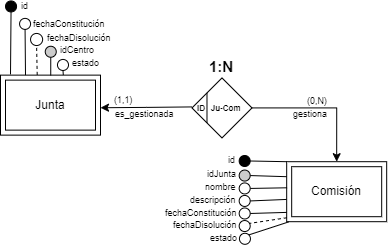
\includegraphics[scale=0.7]{img/diagramas/EER/I-Ju-Com}
        \caption{Interrelación: Junta - Comisión}
        \label{fig:I-Ju-Com}
    \end{figure}
    
    \item \textbf{Ejemplo} (Tabla \ref{table:I-Ju-Com}).

    \begin{table}[H]
    \centering
        \begin{tabular}{ | c | c | c |  }
             \hline
                 \textbf{Entidad} & \textbf{Atributo} & \textbf{Ejemplo}\\       
             \hline
                 \textbf{Junta}  & \underline{id} & 1\\
                  & idCentro & 1\\
                  & fechaConstitución & 10/09/2023\\
                  & fechaDisolución & null\\
                  & estado & 1\\
              \hline
                 \textbf{Comisión}  & \underline{id} & 1\\
                  & id & 1\\
                  & idJunta & 1\\
                  & nombre & Asuntos económicos\\
                  & descripción & Economía de la comisión\\
                  & fechaConstitución & 10/09/2023\\
                  & fechaDisolución & null\\
                  & estado & 1\\
        \end{tabular}
        \caption{Ejemplo de la interrelación \textit{Junta - Comisión}}
        \label{table:I-Ju-Com}
    \end{table}
\end{itemize}

\subsection{Interrelación: Junta - Convocatoria}
\begin{itemize}
    \item \textbf{Nombre}: Ju-Conv.
    \item \textbf{Descripción}: esta interrelación muestra que una junta puede gestionar cero, uno o más convocatorias, pero una convocatoria solamente puede ser gestionada por una junta.
    \item \textbf{Tipo}: la entidad Convocatoria presenta una debilidad por identificación respecto de la entidad Junta.
    \item \textbf{Cardinalidad}. 1:N
    \begin{itemize}
        \item Cardinalidad de Junta (0,n): una junta puede tener asociados 0, 1 o varias convocatorias.
        \item Cardinalidad de Convocatoria (1,1): una convocatoria solamente está asociado a una junta.
    \end{itemize}
    \item \textbf{Atributos}: ninguno
    \item \textbf{Diagrama} (Figura \ref{fig:I-Ju-Conv}) 
    \begin{figure}[H]
        \centering
        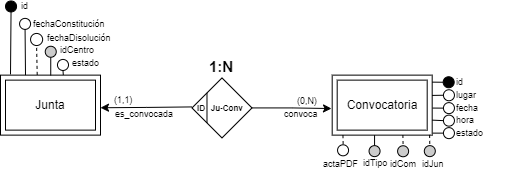
\includegraphics[scale=0.7]{img/diagramas/EER/I-Ju-Conv}
        \caption{Interrelación: Junta - Convocatoria}
        \label{fig:I-Ju-Conv}
    \end{figure}
    
    \item \textbf{Ejemplo} (Tabla \ref{table:I-Ju-Conv}).

    \begin{table}[H]
    \centering
        \begin{tabular}{ | c | c | c |  }
             \hline
                 \textbf{Entidad} & \textbf{Atributo} & \textbf{Ejemplo}\\       
             \hline
                 \textbf{Junta}  & \underline{id} & 1\\
                  & idCentro & 1\\
                  & fechaConstitución & 10/09/2023\\
                  & fechaDisolución & null\\
                  & estado & 1\\
              \hline
                  \textbf{Convocatoria}  & \underline{id} & 1\\
                  & lugar & Rectorado\\
                  & fecha & 23/09/2023\\
                  & hora & 11:30\\
                  & idTipo & 1\\
                  & idComision & null\\
                  & idJunta & 1\\
                  & acta & /resources/actas/1.pdf \\
                  & estado & 1\\
        \end{tabular}
        \caption{Ejemplo de la interrelación \textit{Junta - Convocatoria}}
        \label{table:I-Ju-Conv}
    \end{table}
\end{itemize}

\subsection{Interrelación: Comisión - MiembroComisión}
\begin{itemize}
    \item \textbf{Nombre}: Com-MiCom.
    \item \textbf{Descripción}: esta interrelación muestra que una comisión puede ser representada por cero, uno o más miembros de comisión, pero un miembro de comisión solamente representa una comisión.
    \item \textbf{Tipo}: la entidad MiembroComisión presenta una debilidad por identificación respecto de la entidad Comisión.
    \item \textbf{Cardinalidad}. 1:N
    \begin{itemize}
        \item Cardinalidad de Comisión (0,n): una comisión puede tener asociados 0, 1 o varios miembros de comisión.
        \item Cardinalidad de MiembroComisión (1,1): un miembro de comisión solamente está asociado a una comisión.
    \end{itemize}
    \item \textbf{Atributos}: ninguno
    \item \textbf{Diagrama} (Figura \ref{fig:I-Com-MiCom}) 
    \begin{figure}[H]
        \centering
        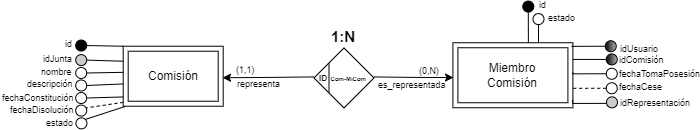
\includegraphics[scale=0.7]{img/diagramas/EER/I-Com-MiCom}
        \caption{Interrelación: Comisión - MiembroComisión}
        \label{fig:I-Com-MiCom}
    \end{figure}
    
    \item \textbf{Ejemplo} (Tabla \ref{table:I-Com-MiCom}).

    \begin{table}[H]
    \centering
        \begin{tabular}{ | c | c | c |  }
             \hline
                 \textbf{Entidad} & \textbf{Atributo} & \textbf{Ejemplo}\\       
             \hline
                 \textbf{Comisión}  & \underline{id} & 1\\
                  & id & 1\\
                  & idJunta & 1\\
                  & nombre & Asuntos económicos\\
                  & descripción & Economía de la comisión\\
                  & fechaConstitución & 10/09/2023\\
                  & fechaDisolución & null\\
                  & estado & 1\\
              \hline
                 \textbf{Miembro Comisión}  & \underline{id} & 1\\
                  & idUsuario & 1\\
                  & idComisión & 1\\
                  & idRepresentación & 2\\
                  & fechaTomaPosesión & 10/09/2023\\
                  & fechaCese & null\\
                  & estado & 1\\
        \end{tabular}
        \caption{Ejemplo de la interrelación \textit{Comisión - MiembroComisión}}
        \label{table:I-Com-MiCom}
    \end{table}
\end{itemize}

\subsection{Interrelación: Comisión - Convocatoria}
\begin{itemize}
    \item \textbf{Nombre}: Com-Conv.
    \item \textbf{Descripción}: esta interrelación muestra que una comisión puede gestionar cero, uno o más convocatorias, pero una convocatoria solamente puede ser gestionada por una comisión.
    \item \textbf{Tipo}: la entidad Convocatoria presenta una debilidad por identificación respecto de la entidad Comisión.
    \item \textbf{Cardinalidad}. 1:N
    \begin{itemize}
        \item Cardinalidad de Comisión (0,n): una comisión puede tener asociados 0, 1 o varias convocatorias.
        \item Cardinalidad de Convocatoria (1,1): una convocatoria solamente está asociado a una comisión.
    \end{itemize}
    \item \textbf{Atributos}: ninguno
    \item \textbf{Diagrama} (Figura \ref{fig:I-Com-Conv}) 
    \begin{figure}[H]
        \centering
        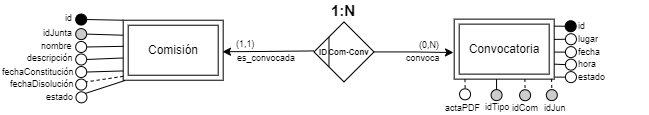
\includegraphics[scale=0.7]{img/diagramas/EER/I-Com-Conv}
        \caption{Interrelación: Comisión - Convocatoria}
        \label{fig:I-Com-Conv}
    \end{figure}
    
    \item \textbf{Ejemplo} (Tabla \ref{table:I-Com-Conv}).

    \begin{table}[H]
    \centering
        \begin{tabular}{ | c | c | c |  }
             \hline
                 \textbf{Entidad} & \textbf{Atributo} & \textbf{Ejemplo}\\       
             \hline
                 \textbf{Comisión}  & \underline{id} & 1\\
                  & id & 1\\
                  & idJunta & 1\\
                  & nombre & Asuntos económicos\\
                  & descripción & Economía de la comisión\\
                  & fechaConstitución & 10/09/2023\\
                  & fechaDisolución & null\\
                  & estado & 1\\
              \hline
                  \textbf{Convocatoria}  & \underline{id} & 1\\
                  & lugar & Rectorado\\
                  & fecha & 23/09/2023\\
                  & hora & 11:30\\
                  & idTipo & 1\\
                  & idComision & null\\
                  & idJunta & 1\\
                  & acta & /resources/actas/1.pdf \\
                  & estado & 1\\
        \end{tabular}
        \caption{Ejemplo de la interrelación \textit{Comisión - Convocatoria}}
        \label{table:I-Com-Conv}
    \end{table}
\end{itemize}

\subsection{Interrelación: Usuario - MiembroGobierno}
\begin{itemize}
    \item \textbf{Nombre}: Usu-MiGob.
    \item \textbf{Descripción}: esta interrelación muestra que un usuario puede corresponder a cero, uno o más miembros de gobierno, pero un miembro de gobierno solamente puede ser un usuario.
    \item \textbf{Tipo}: la entidad MiembroGobierno presenta una debilidad por identificación respecto de la entidad Usuario.
    \item \textbf{Cardinalidad}. 1:N
    \begin{itemize}
        \item Cardinalidad de Usuario (0,n): un usuario puede tener asociados 0, 1 o varias miembros de gobierno.
        \item Cardinalidad de MiembroGobierno (1,1): un miembro de gobierno solamente está asociado a un usuario.
    \end{itemize}
    \item \textbf{Atributos}: ninguno
    \item \textbf{Diagrama} (Figura \ref{fig:I-Usu-MiGob}) 
    \begin{figure}[H]
        \centering
        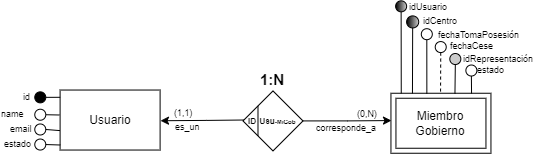
\includegraphics[scale=0.7]{img/diagramas/EER/I-Usu-MiGob}
        \caption{Interrelación: Usuario - MiembroGobierno}
        \label{fig:I-Usu-MiGob}
    \end{figure}
    
    \item \textbf{Ejemplo} (Tabla \ref{table:I-Usu-MiGob}).

    \begin{table}[H]
    \centering
        \begin{tabular}{ | c | c | c |  }
             \hline
                 \textbf{Entidad} & \textbf{Atributo} & \textbf{Ejemplo}\\       
             \hline
                 \textbf{Usuario}  & \underline{id} & 1\\
                  & id & 1\\
                  & name & Manuel Cañas Ramírez\\
                  & email & epsc.director@uco.es\\
                  & password & 2y$10$92IXUNpkjO0rOQ\\
                  & estado & 1\\
              \hline
                  \textbf{Miembro Gobierno}  & \underline{id} & 1\\
                  & idUsuario & 1\\
                  & idCentro & 1\\
                  & idRepresentación & 1\\
                  & fechaTomaPosesión & 10/09/2023\\
                  & fechaCese & null\\
                  & estado & 1\\
        \end{tabular}
        \caption{Ejemplo de la interrelación \textit{Usuario - MiembroGobierno}}
        \label{table:I-Usu-MiGob}
    \end{table}
\end{itemize}

\subsection{Interrelación: Usuario - MiembroJunta}
\begin{itemize}
    \item \textbf{Nombre}: Usu-MiJu.
    \item \textbf{Descripción}: esta interrelación muestra que un usuario puede corresponder a cero, uno o más miembros de junta, pero un miembro de junta solamente puede ser un usuario.
    \item \textbf{Tipo}: la entidad MiembroJunta presenta una debilidad por identificación respecto de la entidad Usuario.
    \item \textbf{Cardinalidad}. 1:N
    \begin{itemize}
        \item Cardinalidad de Usuario (0,n): un usuario puede tener asociados 0, 1 o varias miembros de junta.
        \item Cardinalidad de MiembroJunta (1,1): un miembro de junta solamente está asociado a un usuario.
    \end{itemize}
    \item \textbf{Atributos}: ninguno
    \item \textbf{Diagrama} (Figura \ref{fig:I-Usu-MiJu}) 
    \begin{figure}[H]
        \centering
        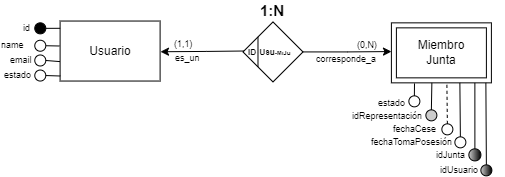
\includegraphics[scale=0.7]{img/diagramas/EER/I-Usu-MiJu}
        \caption{Interrelación: Usuario - MiembroJunta}
        \label{fig:I-Usu-MiJu}
    \end{figure}
    
    \item \textbf{Ejemplo} (Tabla \ref{table:I-Usu-MiJu}).

    \begin{table}[H]
    \centering
        \begin{tabular}{ | c | c | c |  }
             \hline
                 \textbf{Entidad} & \textbf{Atributo} & \textbf{Ejemplo}\\       
             \hline
                 \textbf{Usuario}  & \underline{id} & 1\\
                  & id & 1\\
                  & name & Manuel Cañas Ramírez\\
                  & email & epsc.director@uco.es\\
                  & password & 2y$10$92IXUNpkjO0rOQ\\
                  & estado & 1\\
              \hline
                  \textbf{Miembro Junta}  & \underline{id} & 1\\
                  & idUsuario & 1\\
                  & idJunta & 1\\
                  & idRepresentación & 1\\
                  & fechaTomaPosesión & 10/09/2023\\
                  & fechaCese & null\\
                  & estado & 1\\
        \end{tabular}
        \caption{Ejemplo de la interrelación \textit{Usuario - MiembroJunta}}
        \label{table:I-Usu-MiJu}
    \end{table}
\end{itemize}

\subsection{Interrelación: Usuario - MiembroComisión}
\begin{itemize}
    \item \textbf{Nombre}: Usu-MiCom.
    \item \textbf{Descripción}: esta interrelación muestra que un usuario puede corresponder a cero, uno o más miembros de comisión, pero un miembro de comisión solamente puede ser un usuario.
    \item \textbf{Tipo}: la entidad MiembroComisión presenta una debilidad por identificación respecto de la entidad Usuario.
    \item \textbf{Cardinalidad}. 1:N
    \begin{itemize}
        \item Cardinalidad de Usuario (0,n): un usuario puede tener asociados 0, 1 o varias miembros de comisión.
        \item Cardinalidad de MiembroComisión (1,1): un miembro de comisión solamente está asociado a un usuario.
    \end{itemize}
    \item \textbf{Atributos}: ninguno
    \item \textbf{Diagrama} (Figura \ref{fig:I-Usu-MiCom}) 
    \begin{figure}[H]
        \centering
        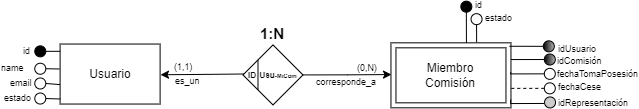
\includegraphics[scale=0.7]{img/diagramas/EER/I-Usu-MiCom}
        \caption{Interrelación: Usuario - MiembroComisión}
        \label{fig:I-Usu-MiCom}
    \end{figure}
    
    \item \textbf{Ejemplo} (Tabla \ref{table:I-Usu-MiCom}).

    \begin{table}[H]
    \centering
        \begin{tabular}{ | c | c | c |  }
             \hline
                 \textbf{Entidad} & \textbf{Atributo} & \textbf{Ejemplo}\\       
             \hline
                 \textbf{Usuario}  & \underline{id} & 1\\
                  & id & 1\\
                  & name & Manuel Cañas Ramírez\\
                  & email & epsc.director@uco.es\\
                  & password & 2y$10$92IXUNpkjO0rOQ\\
                  & estado & 1\\
              \hline
                  \textbf{Miembro Comisión}  & \underline{id} & 1\\
                  & idUsuario & 1\\
                  & idComisión & 1\\
                  & idRepresentación & 1\\
                  & fechaTomaPosesión & 10/09/2023\\
                  & fechaCese & null\\
                  & estado & 1\\
        \end{tabular}
        \caption{Ejemplo de la interrelación \textit{Usuario - MiembroComisión}}
        \label{table:I-Usu-MiCom}
    \end{table}
\end{itemize}

\begin{landscape}
\section{Diagrama del Modelo Entidad-Interrelación}\label{sec:diagrama-E-R}
El diagrama completo se muestra en la figura \ref{fig:EER_v5}
\begin{figure}[H]
    \centering
    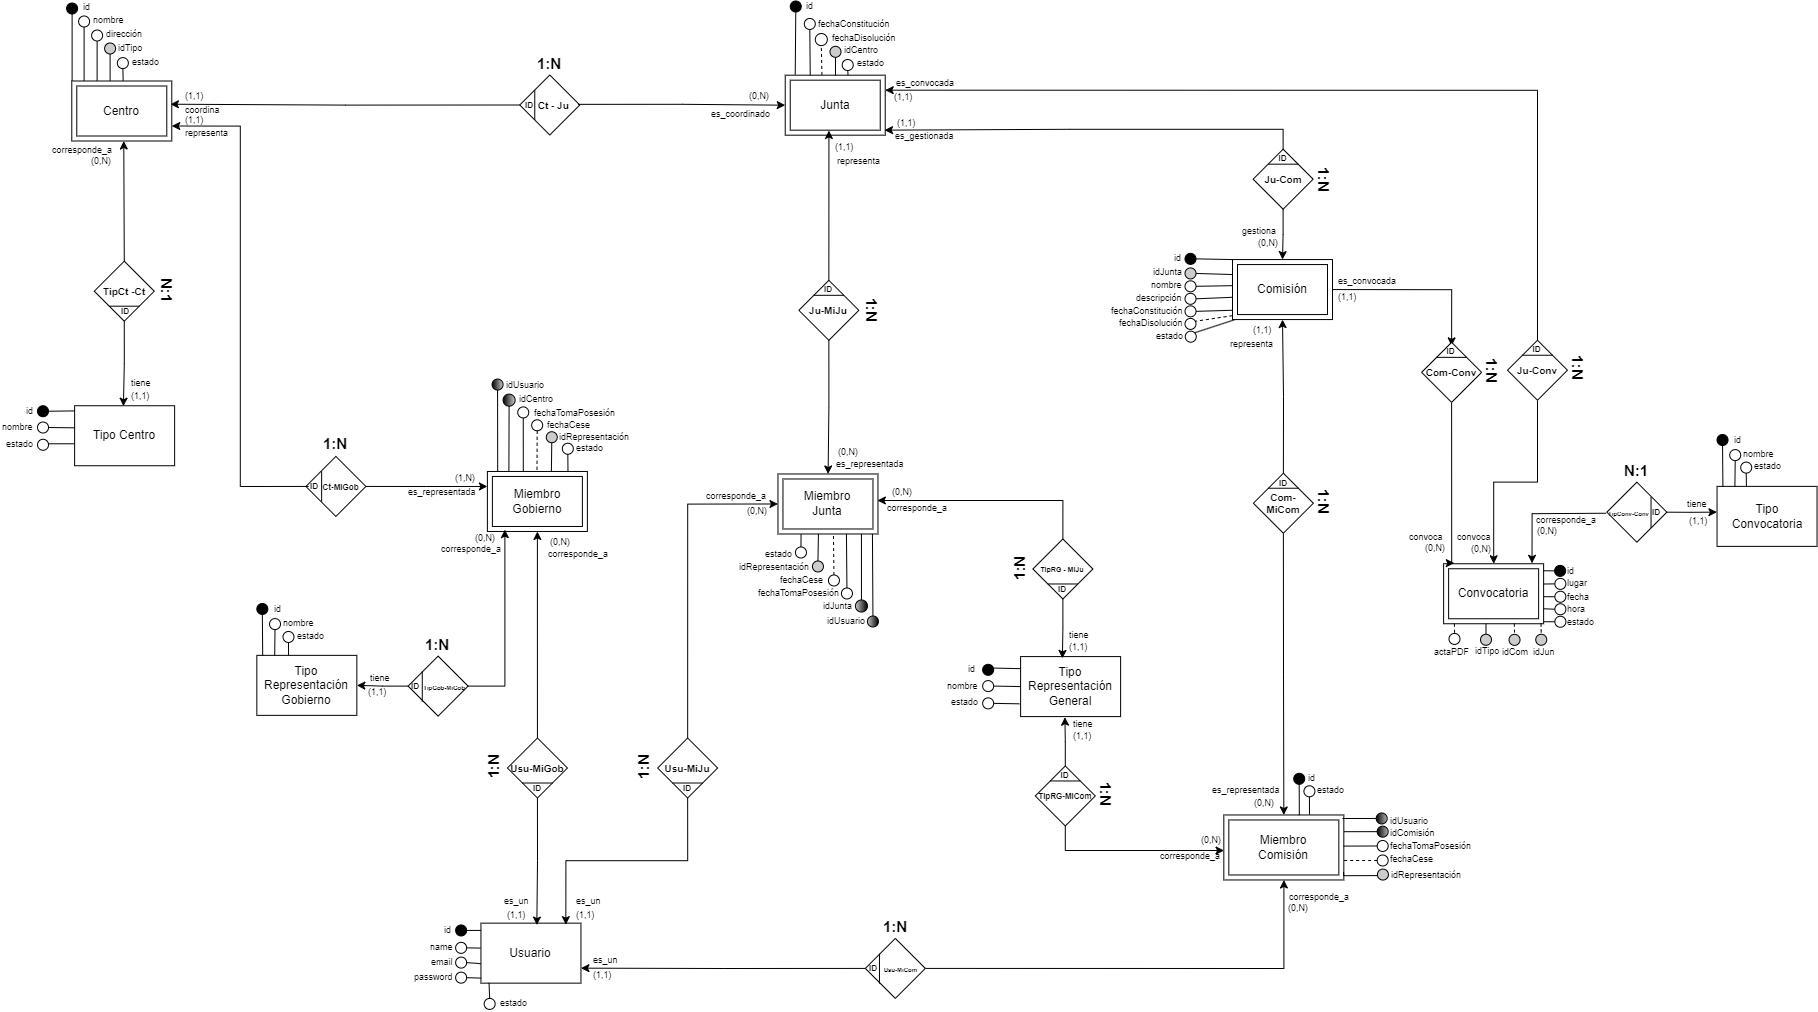
\includegraphics[scale=0.35]{img/diagramas/EER/EER_v5.png}
    \caption{Diagrama del modelo Entidad - Interrelación}
    \label{fig:EER_v5}
\end{figure}
\end{landscape}
